\documentclass{minimal}
\usepackage{graphicx,color}
\usepackage[utf8]{inputenc}
\usepackage[papersize={419.00bp,314.00bp},text={419.00bp,314.00bp}]{geometry}
\begin{document}
\centering
% Title: gl2ps_renderer figure
% Creator: GL2PS 1.4.2, (C) 1999-2020 C. Geuzaine
% For: Octave
% CreationDate: Mon Dec 12 16:45:05 2022
\setlength{\unitlength}{1pt}
\begin{picture}(0,0)
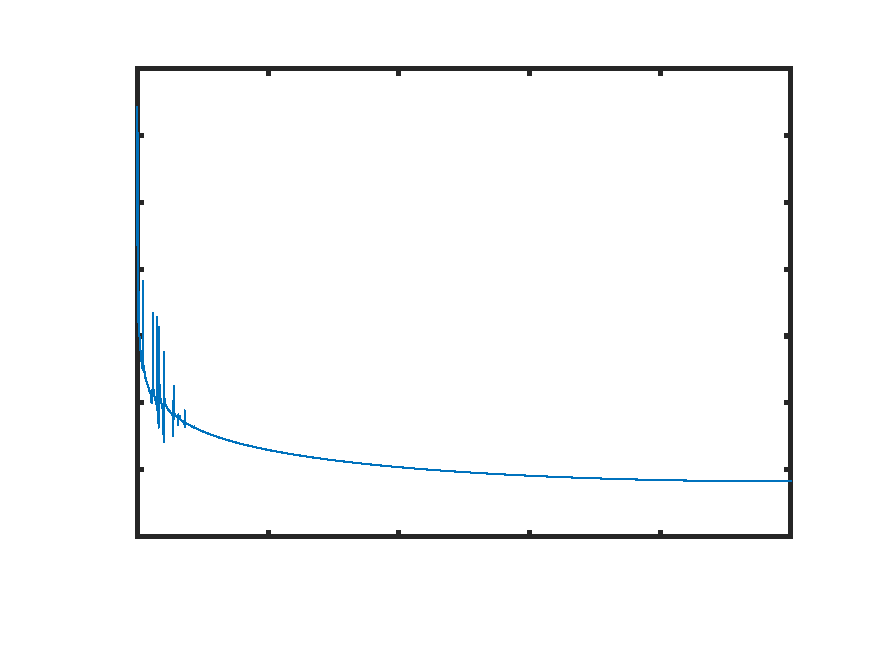
\includegraphics[scale=1]{DoubleKapitzaFourierTheta1-inc}
\end{picture}%
\begin{picture}(419,314)(0,0)
\fontsize{20}{0}\selectfont\put(65.9877,41.4139){\makebox(0,0)[t]{\textcolor[rgb]{0.15,0.15,0.15}{{0}}}}
\fontsize{20}{0}\selectfont\put(128.71,41.4139){\makebox(0,0)[t]{\textcolor[rgb]{0.15,0.15,0.15}{{0.1}}}}
\fontsize{20}{0}\selectfont\put(191.433,41.4139){\makebox(0,0)[t]{\textcolor[rgb]{0.15,0.15,0.15}{{0.2}}}}
\fontsize{20}{0}\selectfont\put(254.155,41.4139){\makebox(0,0)[t]{\textcolor[rgb]{0.15,0.15,0.15}{{0.3}}}}
\fontsize{20}{0}\selectfont\put(316.878,41.4139){\makebox(0,0)[t]{\textcolor[rgb]{0.15,0.15,0.15}{{0.4}}}}
\fontsize{20}{0}\selectfont\put(379.601,41.4139){\makebox(0,0)[t]{\textcolor[rgb]{0.15,0.15,0.15}{{0.5}}}}
\fontsize{20}{0}\selectfont\put(56,56.388){\makebox(0,0)[r]{\textcolor[rgb]{0.15,0.15,0.15}{{-10}}}}
\fontsize{20}{0}\selectfont\put(56,88.4755){\makebox(0,0)[r]{\textcolor[rgb]{0.15,0.15,0.15}{{-5}}}}
\fontsize{20}{0}\selectfont\put(56,120.563){\makebox(0,0)[r]{\textcolor[rgb]{0.15,0.15,0.15}{{0}}}}
\fontsize{20}{0}\selectfont\put(56,152.65){\makebox(0,0)[r]{\textcolor[rgb]{0.15,0.15,0.15}{{5}}}}
\fontsize{20}{0}\selectfont\put(56,184.738){\makebox(0,0)[r]{\textcolor[rgb]{0.15,0.15,0.15}{{10}}}}
\fontsize{20}{0}\selectfont\put(56,216.825){\makebox(0,0)[r]{\textcolor[rgb]{0.15,0.15,0.15}{{15}}}}
\fontsize{20}{0}\selectfont\put(56,248.913){\makebox(0,0)[r]{\textcolor[rgb]{0.15,0.15,0.15}{{20}}}}
\fontsize{20}{0}\selectfont\put(56,281){\makebox(0,0)[r]{\textcolor[rgb]{0.15,0.15,0.15}{{25}}}}
\fontsize{22}{0}\selectfont\put(222.794,21.4139){\makebox(0,0)[t]{\textcolor[rgb]{0.15,0.15,0.15}{{Frequency}}}}
\fontsize{22}{0}\selectfont\put(22,168.694){\rotatebox{90}{\makebox(0,0)[b]{\textcolor[rgb]{0.15,0.15,0.15}{{log(Power Spectra)}}}}}
\fontsize{22}{0}\selectfont\put(222.794,291){\makebox(0,0)[b]{\textcolor[rgb]{0,0,0}{{Power Spectra of $\theta_1$}}}}
\end{picture}
\end{document}
